\documentclass[a4paper,11pt]{jreport}

\usepackage[dvipdfmx]{graphicx}
%% dvipdfmx を使ってPDFの「しおり」を付ける場合
%%\usepackage[dvipdfmx,bookmarks=true,bookmarksnumbered=true,bookmarkstype=toc]{hyperref} \usepackage{pxjahyper}
\usepackage{ulem}
\usepackage{times}
\usepackage[dvipdfmx]{graphicx}
\usepackage{latexsym}
\usepackage[hang,small,bf]{caption}
\usepackage[subrefformat=parens]{subcaption}
\usepackage{listings}
\captionsetup{compatibility=false}

\newcommand\figref[1]{\textbf{図~\ref{fig:#1}}}
\newcommand\tabref[1]{\textbf{表~\ref{tab:#1}}}


\def\Underline{\setbox0\hbox\bgroup\let\\\endUnderline}
\def\endUnderline{\vphantom{y}\egroup\smash{\underline{\box0}}\\}
\def\|{\verb|}
%


\lstset{
  basicstyle={\ttfamily},
  identifierstyle={\small},
  commentstyle={\smallitshape},
  keywordstyle={\small\bfseries},
  ndkeywordstyle={\small},
  stringstyle={\small\ttfamily},
  frame={tb},
  breaklines=true,
  columns=[l]{fullflexible},
  numbers=left,
  xrightmargin=0zw,
  xleftmargin=3zw,
  numberstyle={\scriptsize},
  stepnumber=1,
  numbersep=1zw,
  lineskip=-0.5ex
}

\setcounter{tocdepth}{3}
\setcounter{page}{-1}

\setlength{\oddsidemargin}{0.1in}
\setlength{\evensidemargin}{0.1in} 
\setlength{\topmargin}{0in}
\setlength{\textwidth}{6in} 
%\setlength{\textheight}{10.1in}
\setlength{\parskip}{0em}
\setlength{\topsep}{0em}

%% タイトル生成用パッケージ(重要)
\usepackage{coins-jp}




%% タイトル
\title{非同期I/Oと非同期通信処理を統合管理する\\スケジューリング設計の検討}
%% 著者
\author{前田 椋祐}
%% 指導教員
\advisor{建部 修見}

%% 年度と主専攻名
\fiscalyear{2024}
%\majorfield{ソフトウェアサイエンス主専攻}
% \majorfield{情報システム主専攻}
\majorfield{知能情報メディア主専攻}


\begin{document}

\maketitle

\thispagestyle{empty}


\thispagestyle{empty}
\vspace*{20pt plus 1fil}
\parindent=1zw
\noindent
%%
%% 論文の要旨
%%
\begin{center}
{\Large \bf 要  旨}
\vspace{2cm}
\end{center}
分散ファイルシステム環境下では,各計算ノードに対して膨大な量のI/Oリクエストが発生する.
I/O性能を向上させるためには,非同期I/O APIを活用し,I/Oリクエストを多重化することでオーバーヘッドを削減することが有効である.
しかし,非同期処理の実現において大量のネイティブスレッドを使用することは,リソースの過剰消費につながる可能性がある.
そこで本研究では,少ないスレッド数で効率的なI/Oを実行する手法として,
io\_uringを用いたシングルスレッド環境での非同期I/Oの性能評価を行い,その有効性を検証する.
さらに,I/Oリクエストとio\_uringのスケジューリングを統合した場合の性能評価も行う.

%%%%%
\par
\vspace{0pt plus 1fil}
\newpage

\pagenumbering{roman} % I, II, III, IV 
\tableofcontents
\listoffigures
%\listoftables

\pagebreak \setcounter{page}{1}
\pagenumbering{arabic} % 1,2,3

\chapter{はじめに}

高性能計算(HPC)分野においては,半導体技術の向上に伴う高い計算性能をもつアクセラレータの登場や,
計算システム全体の大規模並列化によって演算性能が飛躍的に向上している.
しかし,ストレージハードウェアの性能向上はそれに追随しておらず,
ファイルI/Oがシステム全体のボトルネックとなるケースが多い.
特に,ファイルI/Oにおける高レイテンシーが計算効率の低下を引き起こし,システム全体の性能向上を阻む要因となっている.
この問題に対処するため,近年ではストレージシステムにおいてI/Oリクエストの非同期化や多重化が活用され,
ファイルI/Oのレイテンシー隠蔽とスループット向上が図られている.

このI/Oの非同期化に関しては,カーネルレベルでの技術として近年注目を集めているのが,io\_uring APIである.
io\_uringは,従来のブロッキングI/Oや従来の非同期I/Oに比べ,効率的に非同期処理を実現し,ストレージアクセスのレイテンシーを効果的に短縮する技術として期待されている.
現在,io\_uringに関連する様々な研究が行われ,その性能や応用可能性が多くの観点から探求されている.

また,近年ではNVMe SSDやPersistent Memoryといった安価かつ高速なストレージデバイスが登場したことで,
計算ノードにもストレージを搭載し,計算ノードでキャッシュファイルシステムを構築することで
ファイルI/Oの高速化をるアプローチが注目されている\cite{chfs}\cite{gekkofs}.
これにより計算ノード自身が一時的にデータを保持でき,ストレージノードへのアクセス頻度を減らすことでI/Oレイテンシーを低減し,全体的なパフォーマンスの向上が期待されている.

このような水平分散ファイルシステムではノード数が増加するに従ってコネクション数は$O(n^2)$の規模で増加し,
各ノードには多量の通信イベントが発生する. このような状況下で効率的なI/O処理を実現するには,
非同期処理を活用する必要があり,適切な非同期通信・非同期I/Oを行うことが肝要である.
そのためには通信イベントとI/Oイベントの非同期スケジューリングを統合することで,より適切な非同期処理を実現できる可能性がある.
通信とI/Oの連携が可能なスケジューリング機構が構築されることで,
膨大な通信量が発生する水平分散ファイルシステムにおいても,従来以上のスループットが確保できると期待される.

加えて,HPC環境においてはCPUコアが多数搭載されており,並列計算を実行するときは多数のスレッドを生成することで
高速な計算処理を実現している.
この際,ファイルシステムが多数のスレッドを生成しI/O処理を行うと,コンテキストスイッチのオーバーヘッドにより,
本来の計算処理に支障をきたす可能性がある.
そのため,できるだけ少ないスレッドで効率的にI/Oを実行することが重要である.

本研究では,HPC環境におけるこのようなストレージ性能の向上を目指し,
非同期I/Oをより活用するかつ,少ないスレッド数での効率的なI/O処理を実現するべく,
軽量スレッドを用いて通信イベントとI/Oイベントの非同期スケジューリングを統合した際の性能を評価する.

\chapter{予備実験: io\_uringの性能評価}
\section{io\_uringのアーキテクチャ}
io\_uringは,Linuxカーネルにおいて効率的な非同期I/Oを実現するために設計されたインターフェースであり,
従来のI/O APIと比較して低レイテンシかつ高スループットなI/O処理を可能にしている.
io\_uringの基本的なアーキテクチャは,ユーザ空間とカーネル空間間で共有されるリングバッファを用いたデータ構造に基づいている.
このリングバッファは,Submission Queue(SQ)とCompletion Queue(CQ)の2つのキューを備えており,それぞれI/Oリクエストの発行と完了通知に使用される.

ユーザ空間のアプリケーションは,I/OリクエストをSQにエントリとして記述し,カーネルはこのSQを監視することでI/O操作を非同期的に実行する.
操作が完了すると,カーネルは結果をCQに書き込み,アプリケーションはこのCQを参照することで完了したI/Oの結果を確認できる.
この非同期処理により,従来のブロッキングI/Oにおいて必要だったシステムコール回数が大幅に削減され,カーネルとのコンテキストスイッチのオーバーヘッドが軽減される.

また,io\_uringはバッチ処理が可能で,複数のI/Oリクエストを一括して発行することができるため,スループットを高めつつレイテンシを抑えることができる.
この特性は,大量のI/Oリクエストが発生するHPC環境やストレージ集約型のアプリケーションにおいて特に効果を発揮する.

\begin{figure}
	\centering
	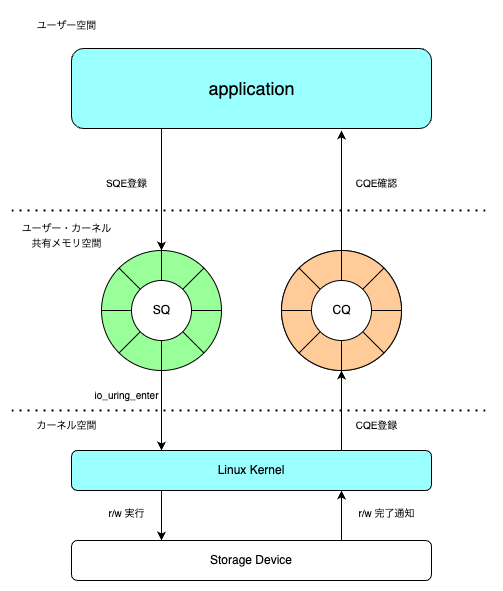
\includegraphics[width=12cm, bb=0 0 503 591]{figures/io_uring_arch.png}
	\caption{io\_uringのアーキテクチャ}
	\label{fig:io_uring}
\end{figure}

%2
\section{io\_uringの性能評価}\label{sec:io_uring_eval}
非同期I/O単体の性能評価を行うために,pwrite/preadとio\_uringの性能測定を行った.
性能評価にはfioのバージョンは3.37を使用し,以下の設定で性能測定を行った.

\begin{itemize}
	\item ファイルサイズ: 100GB
	\item バッファサイズ: 1 〜 1024KiB
	\item io\_depth: 1 〜 256
	\item スレッド数: 1
	\item direct read/write
\end{itemize}

\subsection{実験環境}
本実験では,筑波大学計算科学研究センターで運用中のPegasus スーパーコンピュータを性能評価に用いた.
構成は表\ref{tab:pegasus}の通りである.
実験ではPegasus スーパーコンピュータに搭載されているNVMe SSDを用いており,
I/O性能測定に用いたファイルはノードローカルに搭載されているNVMe SSDにマウントされたxfsファイルシステム上に配置している.


\begin{table*}[ht!]
	\centering
	\caption{Pegasus システムの概要}
	\label{tab:pegasus}
	\hbox to \hsize{\hfil
		\begin{tabular}{l|l}\hline\hline
			CPU          & Intel Xeon Platinum 8468 (48 cores, 1 socket)          \\
			RAM          & 128 GiB, DDR5-4800 16GiB x12 @ 4400 MHz                \\
			% Persistent Memory & 2 TiB,Intel Optane Persistent Memory 300 Series 256 GiB x8 \\
			% GPU               & NVIDIA H100 PCIe x1                                         \\
			NVMe SSD     & 5.4 TiB, RAID-0 @ Micron NVMe 3.2 TB x2, PCIe 4.0 x4   \\
			Interconnect & Mellanox ConnextX-7 InfiniBand NDR200 x1, PCIe 5.0 x16 \\ \hline
		\end{tabular}\hfil}
\end{table*}

\subsection{測定結果}
\subsubsection{bandwidth性能}
pwrite/preadとio\_uringの性能測定結果を\figref{bandwidth}に示す.
sequential read[\figref{seqread}],random read[\figref{randread}]ではpread,io\_uringともにbuffer sizeに対して線形にbandwidthが向上している.
またio\_depthの深さを大きくするにつれbandwidthが向上しており,io\_depthが2以上の場合はpreadよりもio\_uringの方が高いbandwidthを達成しており,
かつより小さいbuffer sizeでHW限界の性能を引き出すことができている.
sequential write[\figref{seqwrite}],random write[\figref{randwrite}]ではreadに比べやや不安定な結果となっているが,
io\_depthが4以上の場合はreadと同じくpwriteに比べio\_uringの方が高いbandwidthを達成していることがわかる.

\begin{figure*}[t]
	\begin{tabular}{cc}
		\begin{minipage}[t]{0.45\hsize}
			\centering
			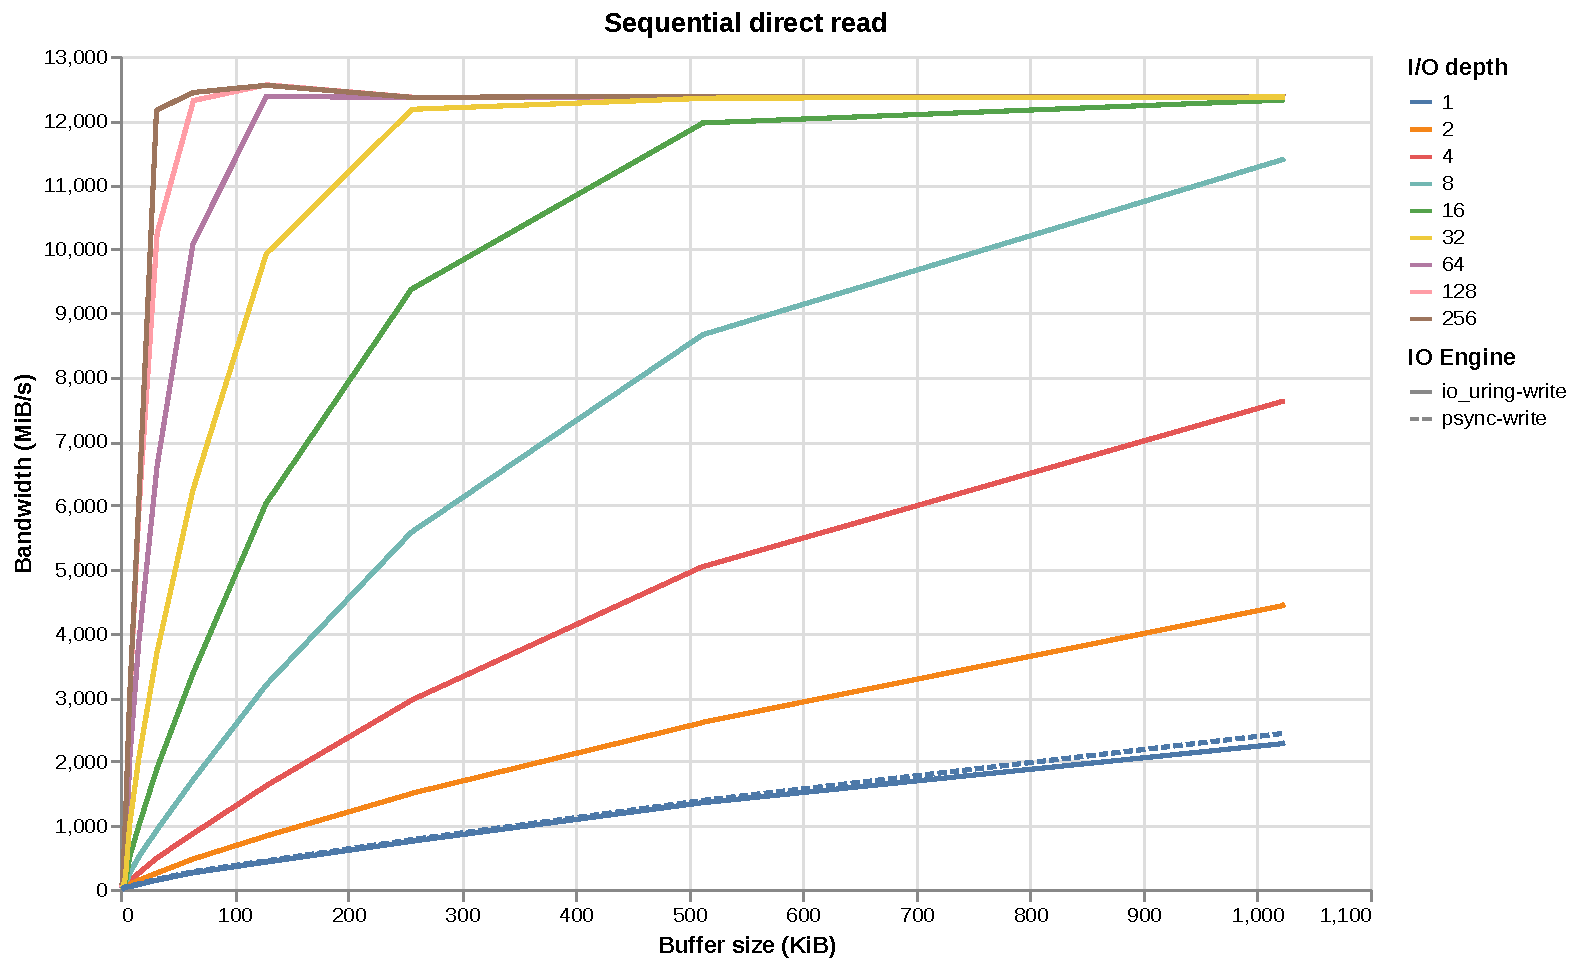
\includegraphics[width=9cm, bb=0 0 800 550]{figures/bw_result_seqr_job1.pdf}
			\subcaption{sequential read}
			\label{fig:seqread}
		\end{minipage} & 
		\begin{minipage}[t]{0.45\hsize}
			\centering
			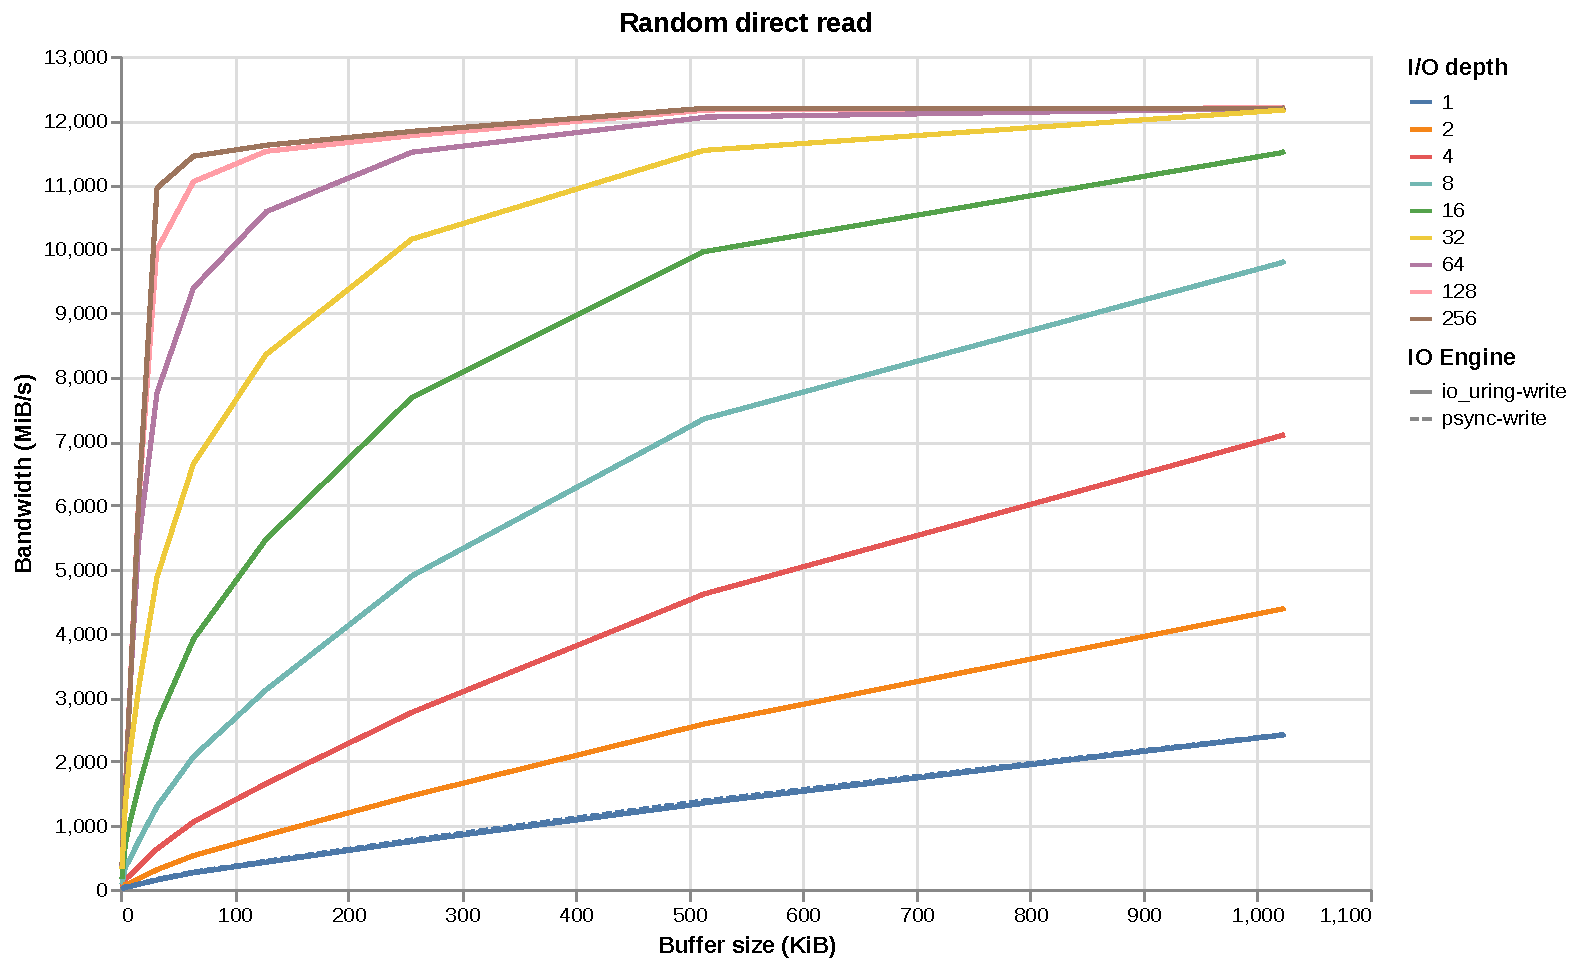
\includegraphics[width=9cm, bb=0 0 800 550]{figures/bw_result_randr_job1.pdf}
			\subcaption{random read}
			\label{fig:randread}
		\end{minipage} \\
		
		\begin{minipage}[t]{0.45\hsize}
			\centering
			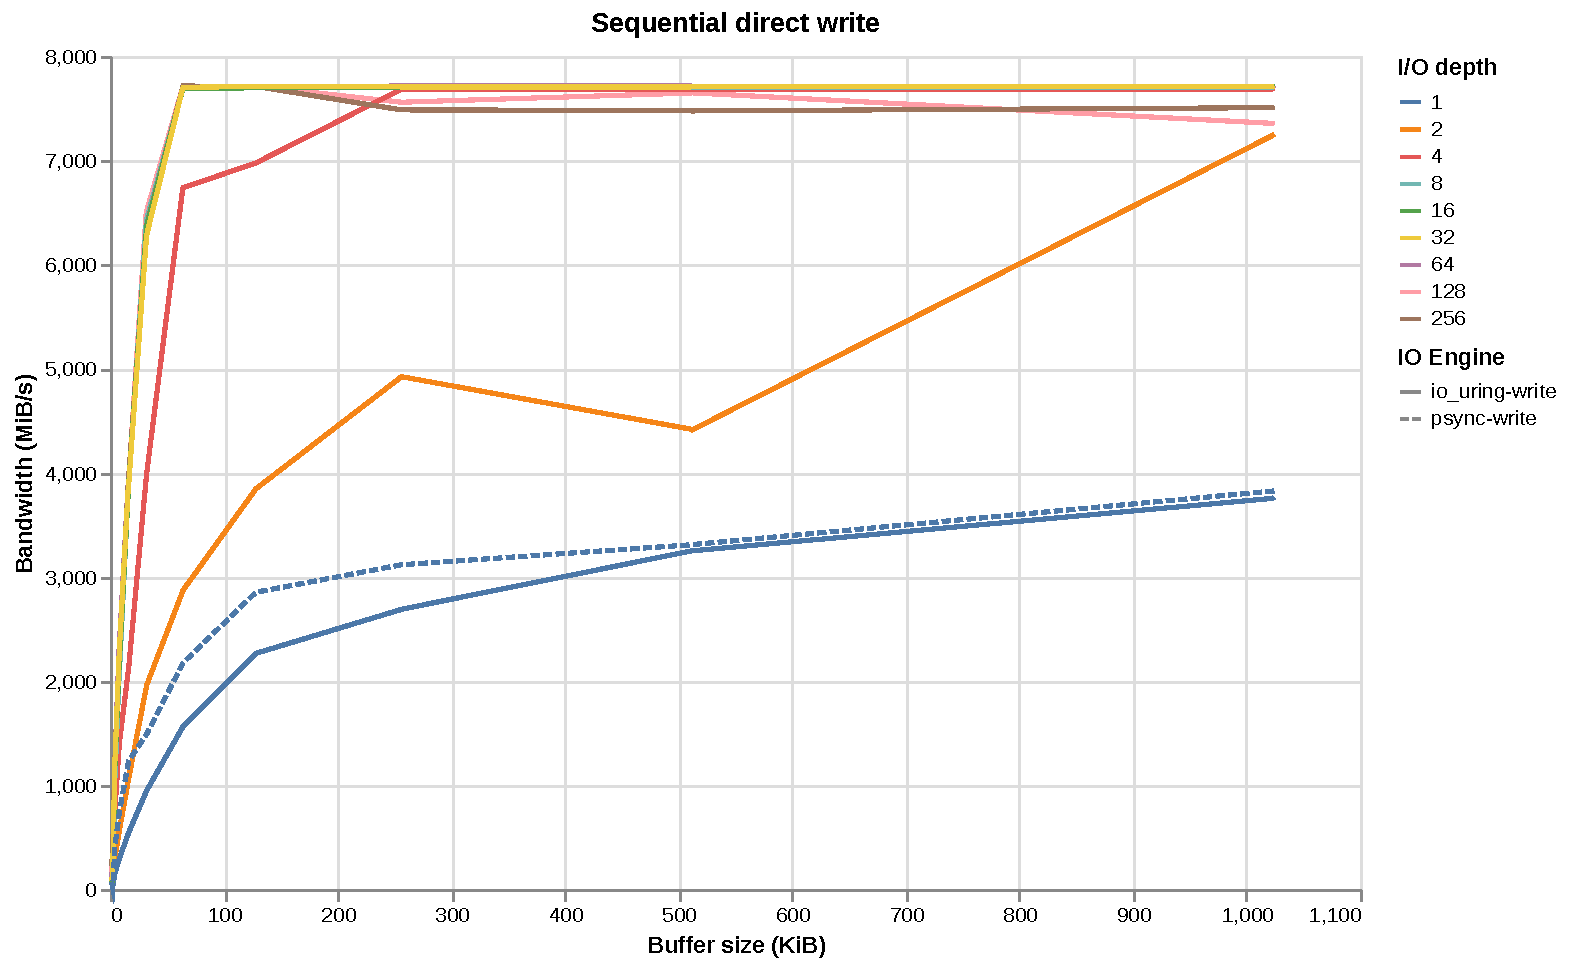
\includegraphics[width=9cm, bb=0 0 800 550]{figures/bw_result_seqw_job1.pdf}
			\subcaption{sequential write}
			\label{fig:seqwrite}
		\end{minipage} & 
		\begin{minipage}[t]{0.45\hsize}
			\centering
			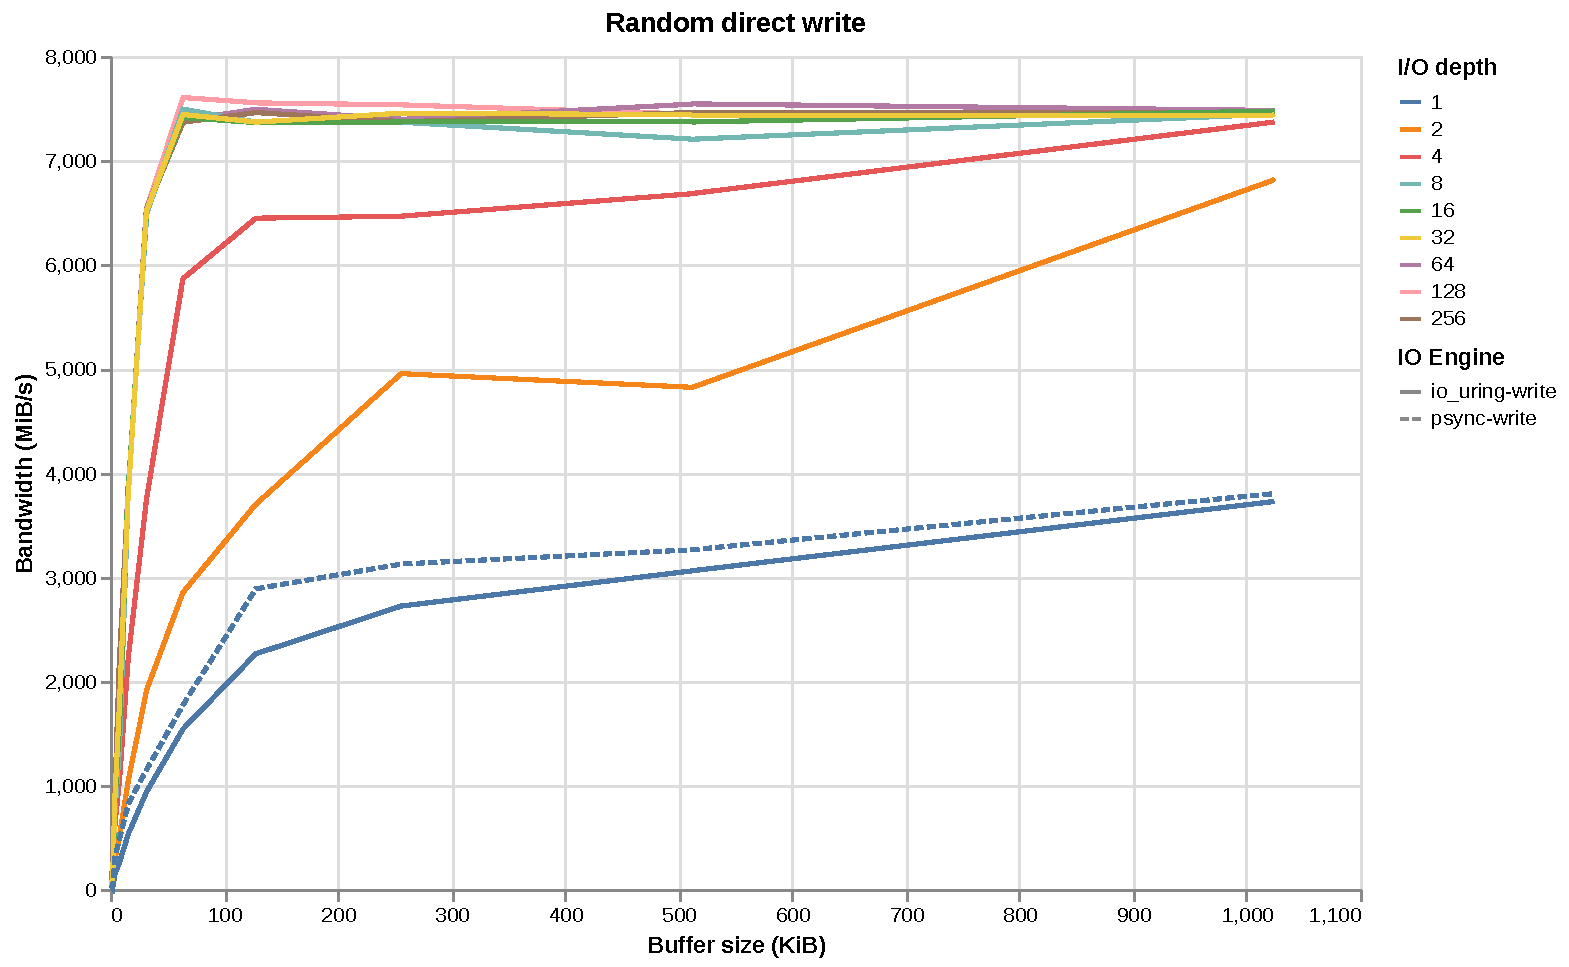
\includegraphics[width=9cm, bb=0 0 800 550]{figures/bw_result_randw_job1.pdf}
			\subcaption{random write}
			\label{fig:randwrite}
		\end{minipage}
	\end{tabular}
	\caption{I/O性能測定結果}
	\label{fig:bandwidth}
\end{figure*}

\subsubsection{CPU効率}
次に,CPU使用率に対するbandwidthの関係を\figref{cpu}に示す.
グラフの性質としては\figref{bandwidth}と殆ど変わらない結果となっているが,
readではio\_uringはbuffer sizeが1024KiBに至るまで線形に性能が向上している一方,
preadはbuffer sizeが128KiBを超えると傾きが緩やかになっており,性能向上率が低下していることがわかる.
これは,preadではカーネルのメモリ空間にブロックデバイスから読み込んだデータを配置した後,
ユーザーのメモリにメモリコピーが発生し,buffer sizeが大きくなればなるほどメモリコピーのオーバーヘッドが大きくなるためであると考えられる.
またread/write共にbuffer sizeが小さい場合はI/Oに対するCPU効率自体は大きな差はないが,
bandwidthの値はio\_uringの方が高くなっている.
このことから,io\_uringはpread/pwriteに比べてCPU使用率を高い状態でI/Oを実行していることがわかる.

\begin{figure*}[t]
	\begin{tabular}{cc}
		\begin{minipage}[t]{0.45\hsize}
			\centering
			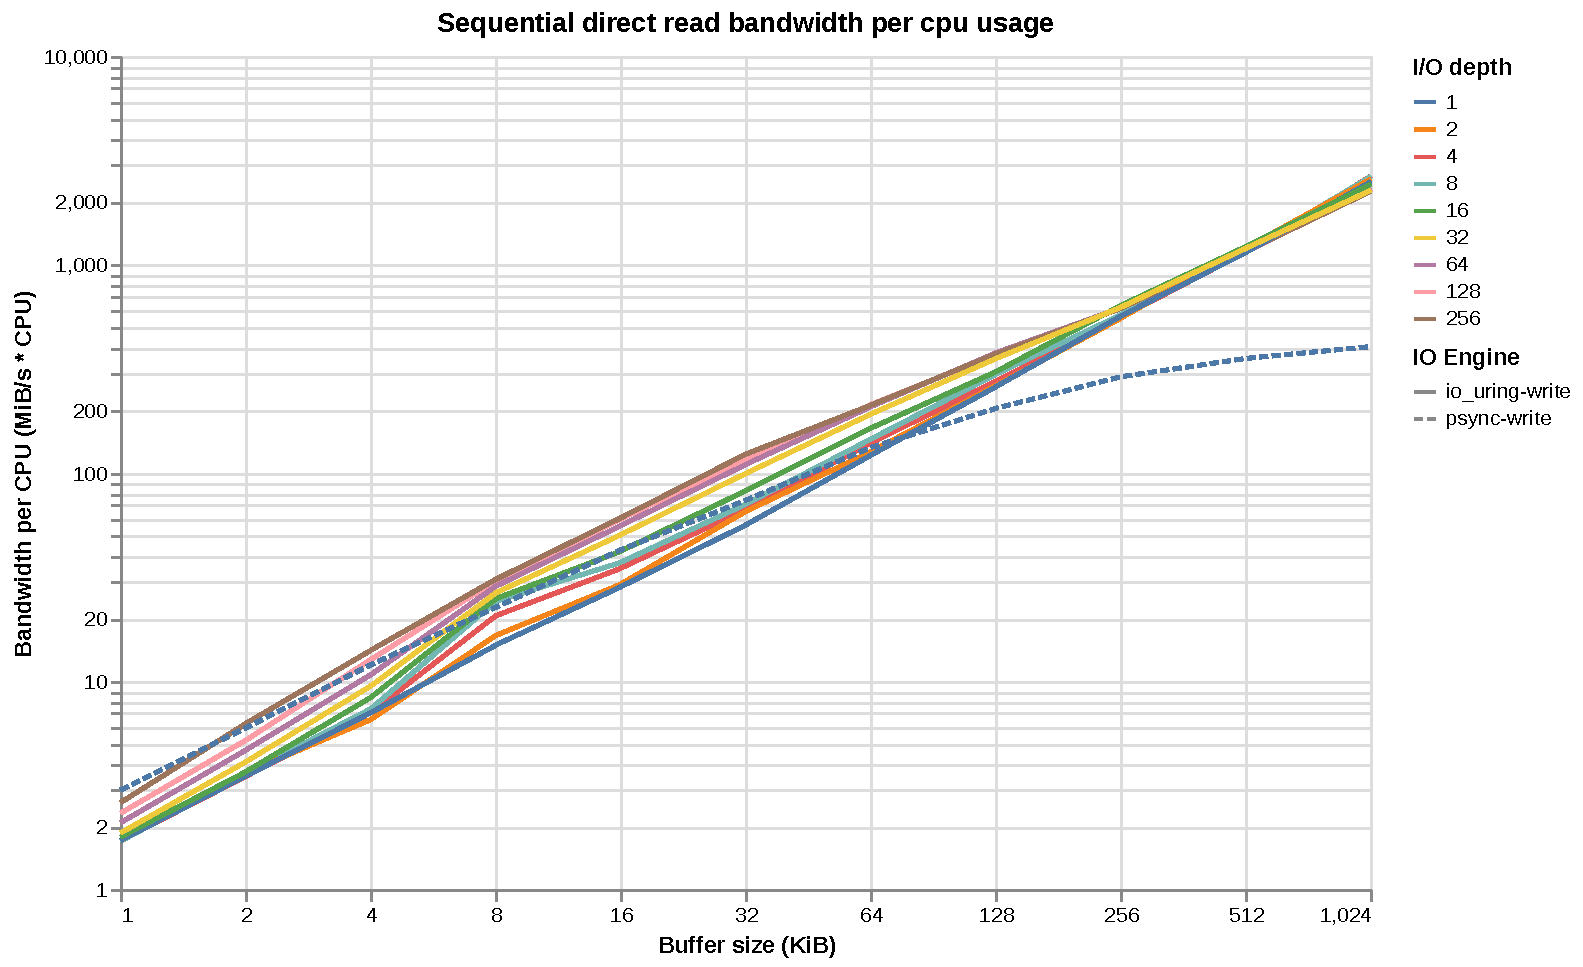
\includegraphics[width=9cm, bb=0 0 800 550]{figures/per_bw_cpu_usage_result_seqr_job1.pdf}
			\subcaption{sequential read}
			\label{fig:seqreadcpu}
		\end{minipage} & 
		\begin{minipage}[t]{0.45\hsize}
			\centering
			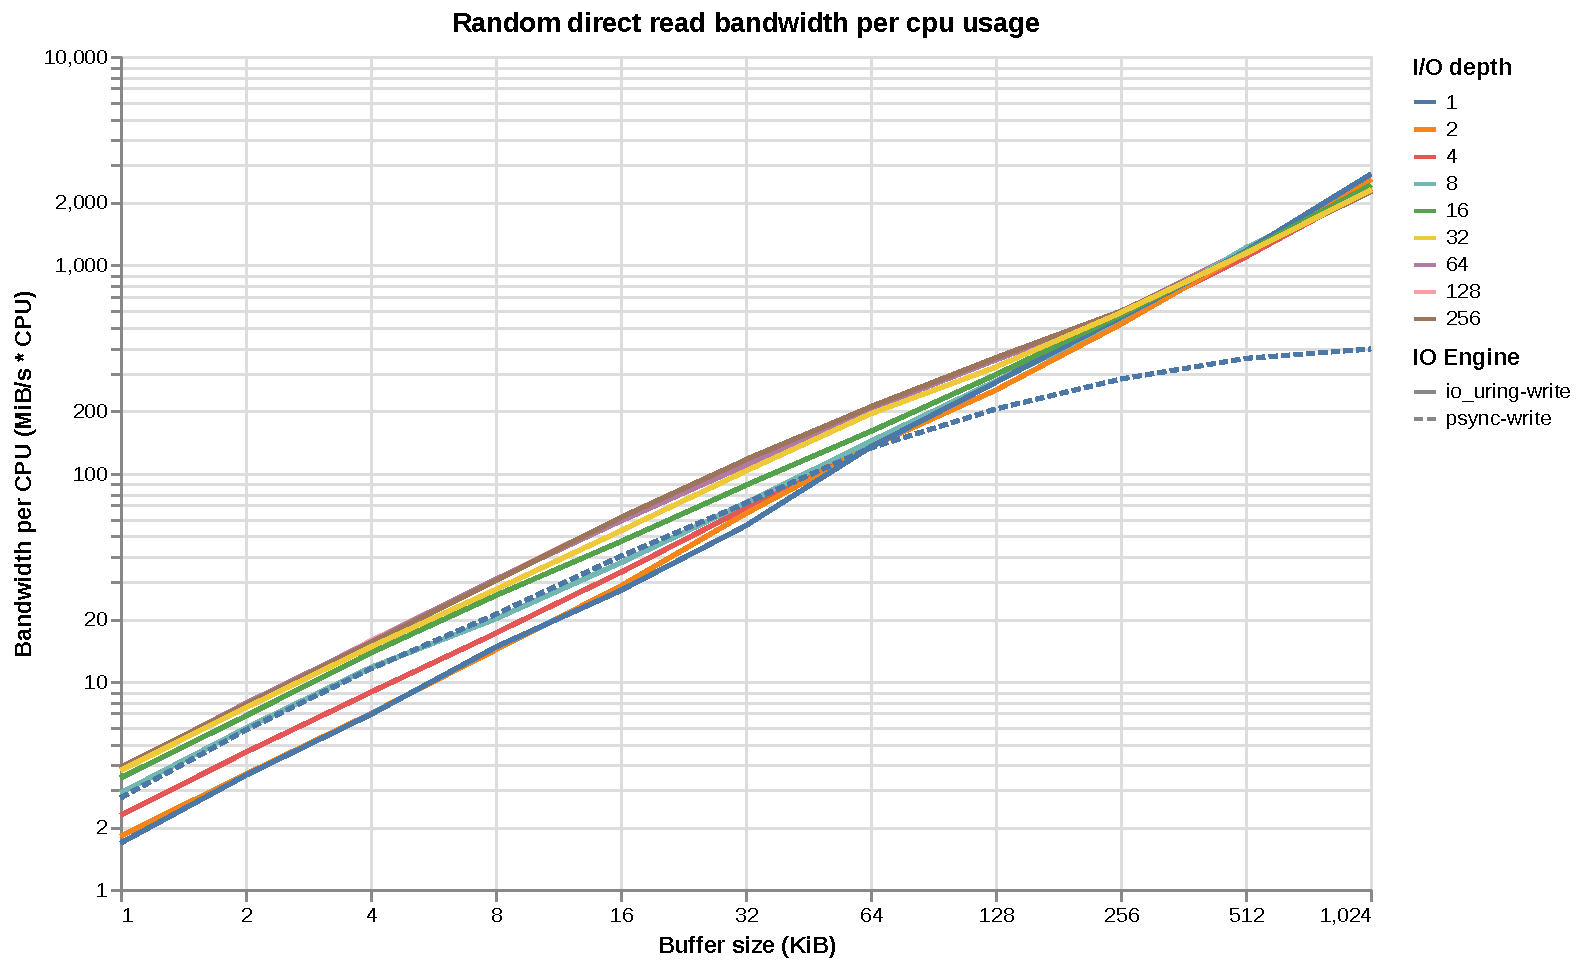
\includegraphics[width=9cm, bb=0 0 800 550]{figures/per_bw_cpu_usage_result_randr_job1.pdf}
			\subcaption{random read}
			\label{fig:randreadcpu}
		\end{minipage} \\
		
		\begin{minipage}[t]{0.45\hsize}
			\centering
			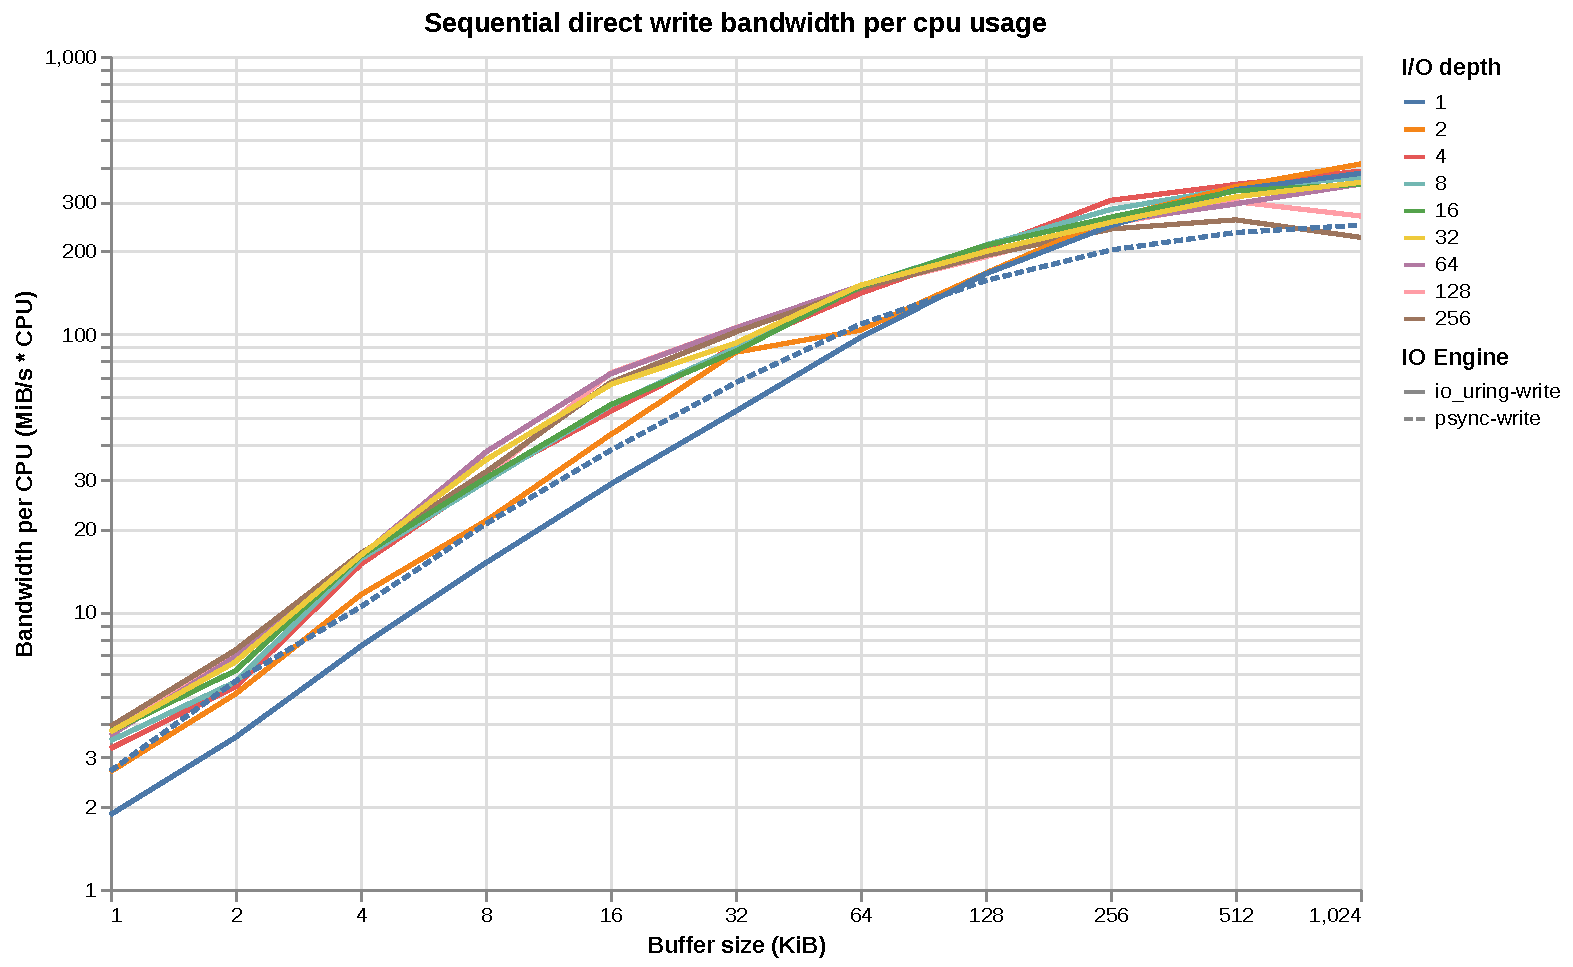
\includegraphics[width=9cm, bb=0 0 800 550]{figures/per_bw_cpu_usage_result_seqw_job1.pdf}
			\subcaption{sequential write}
			\label{fig:seqwritecpu}
		\end{minipage} & 
		\begin{minipage}[t]{0.45\hsize}
			\centering
			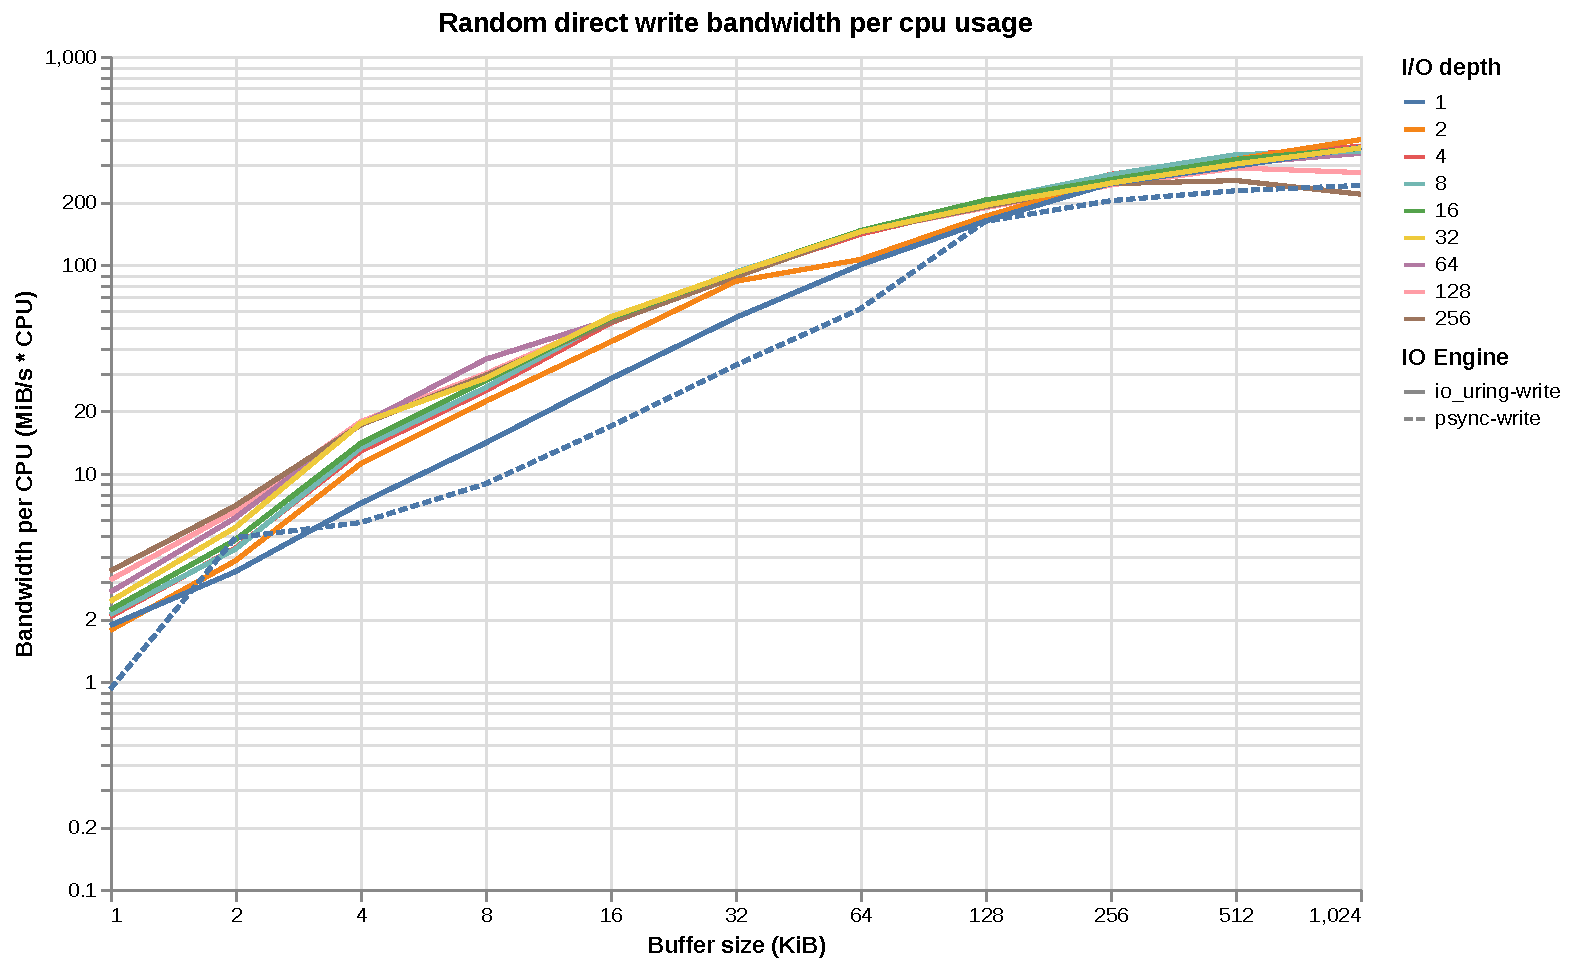
\includegraphics[width=9cm, bb=0 0 800 550]{figures/per_bw_cpu_usage_result_randw_job1.pdf}
			\subcaption{random write}
			\label{fig:randwritecpu}
		\end{minipage}
	\end{tabular}
	\caption{bandwidth / CPU使用率}
	\label{fig:cpu}
\end{figure*}


\subsection{考察}
本実験では,io\_uringを用いた非同期I/Oの性能評価を行った.
その結果io\_uringはpread/pwriteに比べ同等か,勝る性能を示していることがわかった.
これはpread/pwriteに比べio\_uringはシステムコールの呼び出し回数が少なく,
カーネル・ユーザ間のコンテキストスイッチが少ないためであると考えられる.

また,今回の実験環境として用いたNVMe SSDの性能特性として,
NVMeコマンドのキューイング機能を活用することでI/O性能を向上させることができるため,
io\_uringのような非同期I/O APIを用いることでNVMe SSDの性能を最大限引き出すことができていると考えられる.

加えてCPU効率においては,バッファサイズが小さいときはio\_uringとpread/pwriteに大きな差はないが,
バッファサイズが大きくなるにつれio\_uringの方がCPU効率が高いことがわかった.
これにより,io\_uringを用いると,より少ないスレッド数でI/O処理を行うことができるため,
HPC環境においては,多数のスレッドを生成することで発生するコンテキストスイッチのオーバーヘッドを軽減することができると考えられる.

\chapter{提案手法}
\section{Rust async/await}
Rustの非同期処理機構\cite{rust-async-rfc}は,Futureというインターフェースを実装したステートマシンによるグリーンスレッドによって実現されている.
Rust言語ではFutureインターフェースやその糖衣構文であるasync/awaitのみが言語仕様として定義されており,
スケジューリングや実行はサードパーティのライブラリに依存している.
サードパーティ実装としては以下のものが挙げられる.

\begin{itemize}
	\item tokio
	\item async-std
	\item smol
	\item glommio
	\item monoio
\end{itemize}

Rustの言語機能として搭載されているasync/await構文はそれぞれFutureインターフェースの宣言,pollの実行に対応しており,
async構文を用いた関数は\figref{fig:async}のようにRustコンパイラは解釈する.

% \begin{lstlisting}[caption=async構文の解釈, label=lst:async]
% // async構文を用いた関数
% async fn foo() -> u32 {
%   1
% }

% // async構文を使わない場合の表現
% fn foo() -> impl Future<Output = u32> {
%   std::future::ready(1)
% }
% \end{lstlisting}

\begin{figure}[tb]
	\centering
	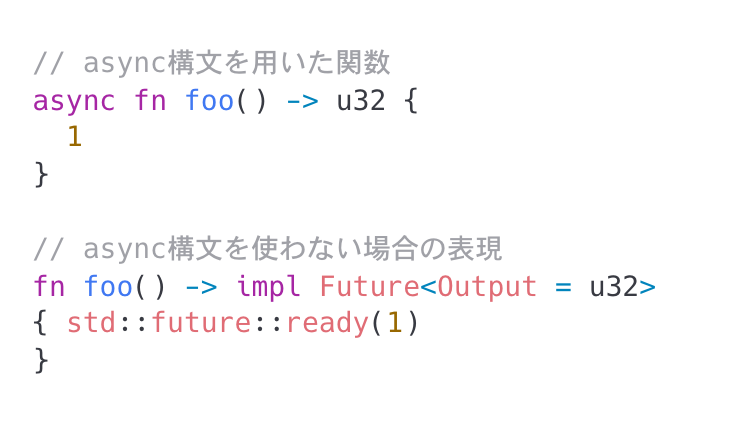
\includegraphics[width=9cm, bb=0 0 800 550]{figures/async_future.png}
	\caption{async構文の解釈}
	\label{fig:async}
\end{figure}

impl構文は,関数の戻り値がtraitを実装している構造体を返すことを示しており,
この場合はFutureインターフェースを実装した構造体を返すことを示している.

また,戻り値がFutureとなっているような関数を定義した場合,
Rustコンパイラはコンパイル時にFutureインターフェースを実装したステートマシン構造体を戻り値として返すように変換する.
この構造体はローカル変数をフィールドとして持つことで,再配置されても関数の実行が継続できるようになっており,
Rustの非同期処理におけるグリーンスレッドとしての役割を担っている. 

Futureインターフェースは,pollというメソッドを定義しており,
\figref{fig:future}に示すようなインターフェースとなっている.
\begin{figure}[tb]
	\centering
	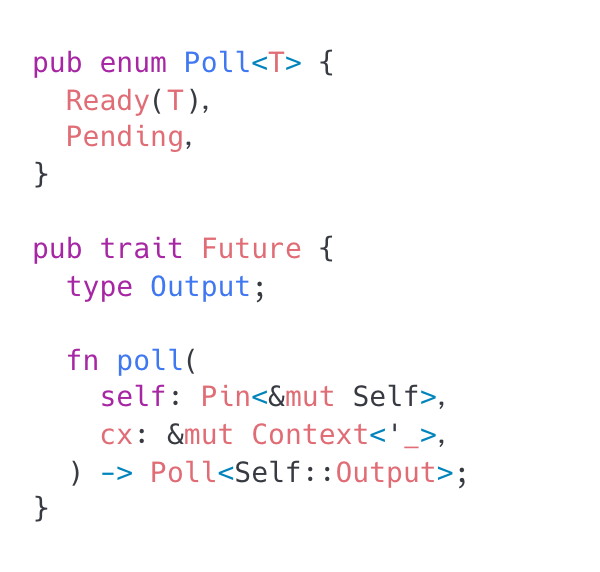
\includegraphics[width=9cm, bb=0 0 800 550]{figures/future_trait.png}
	\caption{async構文の解釈}
	\label{fig:future}
\end{figure}
pollメソッドを呼び出すことでFutureを実行することができ,
Futureの実行結果はPoll列挙型で返される.
Readyの場合はFutureが完了し,処理結果が返される.
Pendingの場合はFutureが完了していないことを示し,pollメソッドを再度呼び出すことでFutureを再開する.
await構文はpollメソッドを呼び出す処理を糖衣構文として提供しており,
Pendingの場合はpollメソッドを再度呼び出す処理を非同期的に行うことができる.

サードパーティのライブラリでは主にReactorとExecutorという
2つのコンポーネントを実装することでスケジューリングと実行を行っている.

Executor,Reactorを含めたランタイム全体の概略を\figref{fig:runtime}に示す.
\begin{figure}[tb]
	\centering
	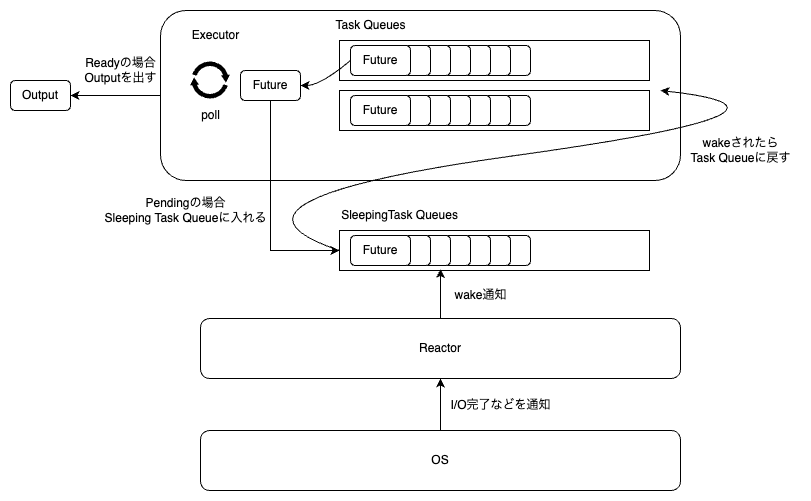
\includegraphics[width=9cm, bb=0 0 800 550]{figures/rust_async.png}
	\caption{Rust 非同期ランタイム概略}
	\label{fig:runtime}
\end{figure}
ExecutorとはFutureを実行するための仕組みである.
複数のTask Queueを持ち,Queueに存在するFutureに対してpollメソッドを呼び出すことでFutureを実行する.
pollメソッドの実行結果がPoll::Pendingの場合は,Sleeping Task QueueにFutureを移動し,
後述のReactorによってTask Queueに戻されるまでFutureの実行を停止する.

ReactorとはI/Oなどのプロセス外部のイベントを監視し,Executorに通知する仕組みである.
OSからのイベント通知を受け取り,Executorに通知することでFutureの再開を行う.

また,Rustの多くの非同期ランタイムでは通信やI/Oなどの重い処理のスケジューリングを
効率的に行うためのAPIを提供しており,
これらのAPIを用いることで,ユーザは非同期処理をより効率的に実装することができる.

\section{glommio}
glommio~\cite{glommio}はDatadog社によって開発されたRustの非同期ランタイムライブラリであり,
I/O処理が全てio\_uring APIを通じて行われることが特徴である.

glommioでは非同期処理の実行を\lstinline|LocalExecutor|という構造体を用いて行う.
\lstinline|LocalExecutor|は,単一のネイティブスレッド上でFutureを実行するための構造体であり,
スレッド間でのFutureの移動が発生しない.
また,glommioはランタイムを生成する際にmain ring,latency ring,poll ringの
三つのio\_uring ring bufferを生成し,I/Oの規模によってそれぞれのring bufferを使い分けることで,
I/Oのスケジューリングを効率的に行うことができる.
加えて,I/Oのbufferを割り当てる際に,独自のメモリアロケータを用いており,
状況に応じてio\_uring APIで確保するbufferとmmapを用いて確保するbufferを使い分けることでもI/O性能を向上させている.

\section{UCX}
UCX(Unified Communication X)は,HPC環境において高性能な通信を実現するためのオープンソースライブラリである.
高度に抽象化されたAPIを通じて,RDMAやTCPなどの通信プロトコルを透過的に利用することができる.
また,UCXは非同期通信をサポートしており,ノンブロッキングAPIを用いることで非同期処理を実現することが可能である.

\section{async-ucx}
async-ucx~\cite{async-ucx}はSuperFSの研究チームによって開発された,
UCXの非同期APIをRustのFutureインターフェースから呼び出せるようにラップしたライブラリである.
Rustの型システムとの整合を実現しており,リソースの自動解放にも対応している.


\section{通信イベントとI/Oイベントの非同期スケジューリング統合方針}\label{sec:policy}
通信イベントとI/Oイベントの非同期スケジューリングの統合方針について述べる.
本研究では,通信イベントとI/OイベントをRust Futureインターフェースによって抽象化し,
単一の非同期ランタイム上で同時にスケジューリングを行うことで,非同期スケジューリングの統合を実現する.
% RDMAやTCPを透過的なインターフェースを通じて通信可能なライブラリであるUCXを
% Rustの非同期インターフェースから呼び出せるようラップした
% async-ucx\cite{async-ucx}ライブラリを用いて通信を行い,
% I/O APIの呼び出しと非同期スケジューリングの統合に後述するRust製非同期ランタイムであるglommioと,



\section{通信イベントとI/Oイベントの非同期スケジューリング統合した際の性能評価}\label{sec:io_rpc_eval}
第\ref{sec:policy}節で述べた方針に基づき,通信イベントとI/Oイベントの非同期スケジューリングを統合し,その性能評価を行う.

\subsection{設計}\label{sec:io_rpc_benchprog}
ベンチマークプログラムの概要を\figref{fig:benchmark}に示す.
\begin{figure}[tb]
	\centering
	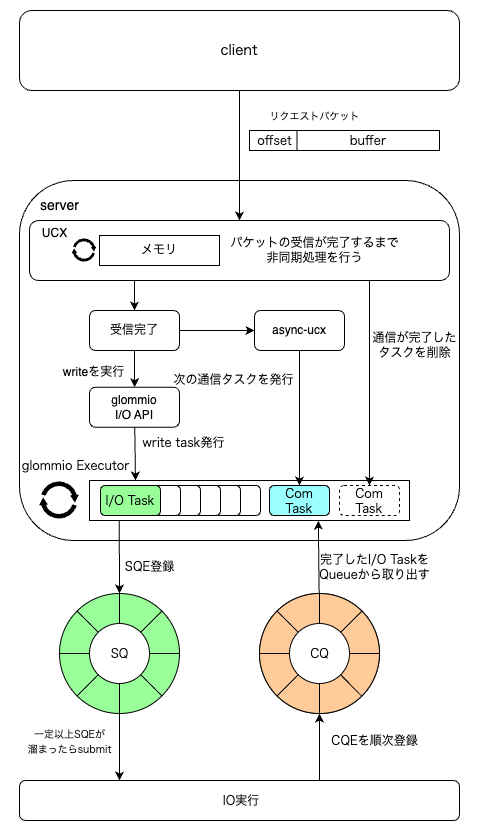
\includegraphics[width=9cm, bb=0 0 520 710]{figures/rpc_overview.png}
	\caption{ベンチマークプログラムの概要}
	\label{fig:benchmark}
\end{figure}

UCXとio\_uringの非同期処理の統合を,async-ucxとglommio I/O APIの関数呼び出しをawaitし,
単一のglommioランタイム上で同時にスケジューリングすることで実現している.

ベンチマークプログラムは主にClientとServerの二つで構成され,それぞれ単一のエンドポイントを持つ.
今回の実験では,データ部のBufferにOffset 8byteを加えたバイナリデータを一つのパケットとし,
パケット一つに対して一つのWrite I/Oイベントと対応づけて実装を行った.

ClientはServerに対して,一回の送信ごとにバッファサイズ分ずらしたoffsetをパケットに含め,Serverにループ処理でパケットを送信しつづける.
ServerはClientから受信したデータをoffset部,data部に分け,
パケット一つごとにwriteを実行するFutureタスクをタスクキューに追加し,
追加したタスク内で指定したファイルのoffset位置にdata部を書き込む.

これらの処理をファイルサイズをバッファサイズで割った回数だけ繰り返し,
ファイルの先頭から書き込みを始めファイルの末尾まで到達した時点での処理時間をRustの\lstinline|std::time::Instant|を用いて計測した.

また,リクエスト単体での性能も測定するため,I/Oを行わずに通信のみを行い,通信後bufferを破棄する処理も実装した.

\subsection{実験環境}
第\ref{sec:io_uring_eval}節と同様に,筑波大学計算科学研究センターで運用中のPegasus スーパーコンピュータを性能評価に用いた.
性能測定の際は2ノード間でそれぞれClientとServerプログラムを実行し,Server側ノードのスクラッチ領域にファイルを作成し,そのファイルに対してダイレクトI/Oを行った.

ファイルサイズはバッファサイズ1024KiBから32KiBまでは128GiBで,16KiBから4KiBまでは16GiBで測定を行った.
バッファサイズ16KiB以降でファイルサイズを16GiBと設定したのは,
バッファサイズが16KiBより小さい場合にファイルサイズ128GiBで測定を実行すると,
プロセスのメモリ使用量が肥大化してしまいノードのメモリを使い切ってしまう事象が発生したためである.

\subsection{測定結果}\label{sec:io_rpc_result}
\subsubsection{Bandwidth性能}
Bandwidth性能の測定結果をfioでベンチしたpsyncとio\_uringの場合,リクエストのみで実行した場合,通信イベントとI/Oイベントを統合した場合それぞれに関して,
\figref{fig:io_rpc_bw}に示す.

\begin{figure}[tb]
	\centering
	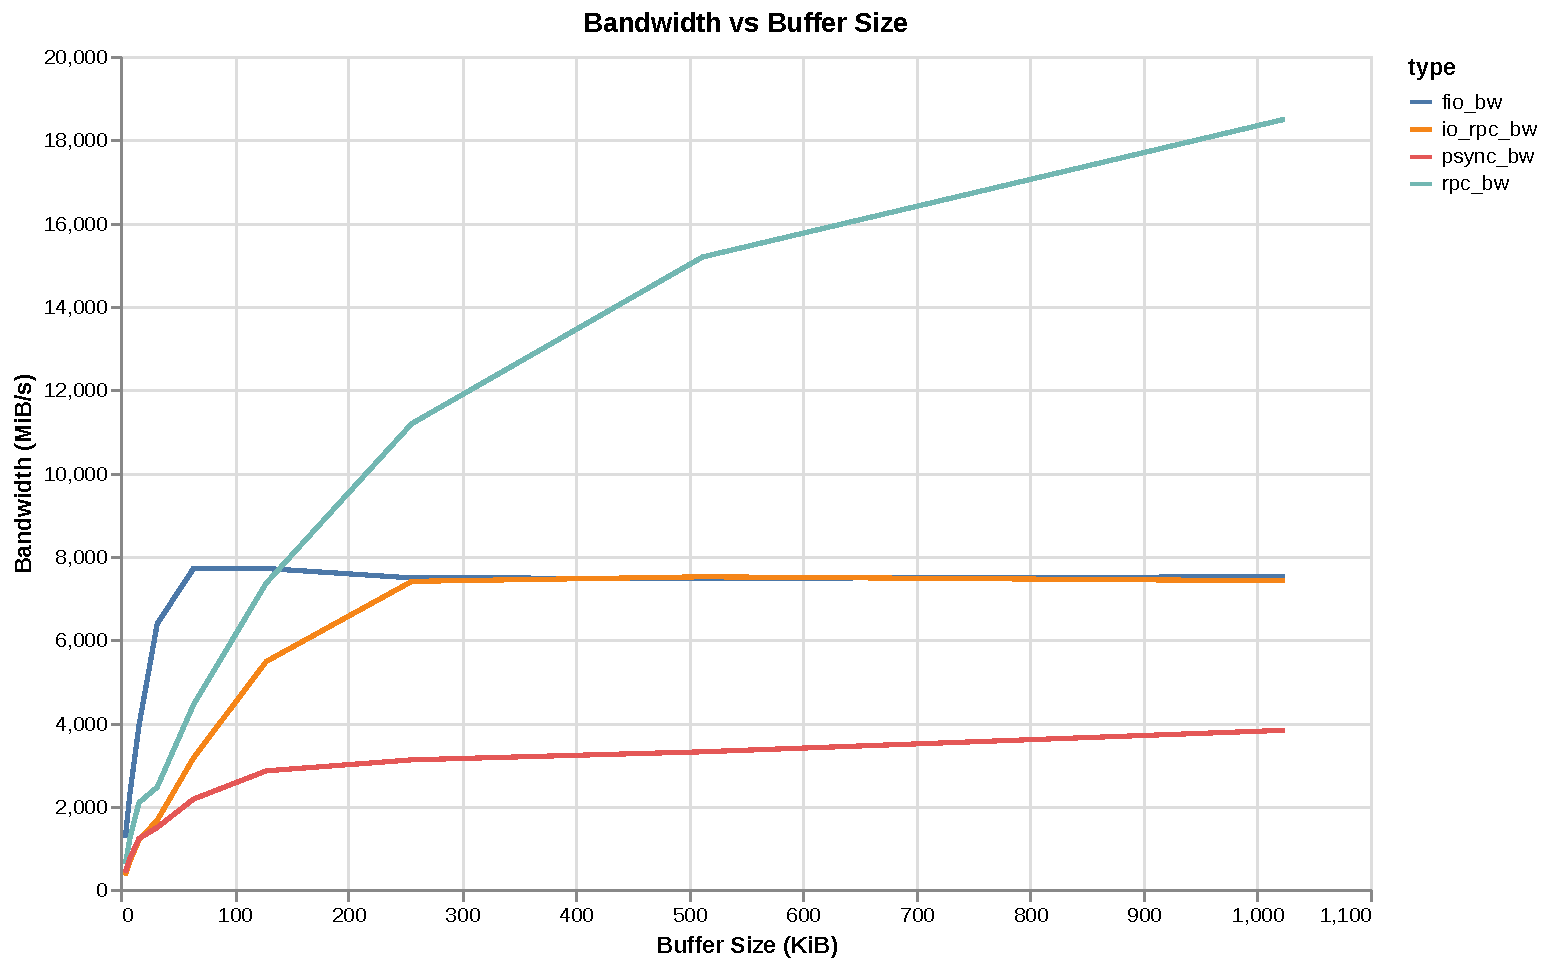
\includegraphics[width=7.5cm, bb=0 0 700 450]{figures/bw_linear_plot.pdf}
	\caption{bandwidth性能}
	\label{fig:io_rpc_bw}
\end{figure}

fioの結果,リクエストのみ,通信・I/O統合の順に傾きが小さくなり,バッファサイズに対するBandwidthの上昇幅が小さくなっていることがわかる.
またHW限界に律速されていない16KiB以下のバッファサイズの結果を見ると,
fioの結果に比べて通信・I/O統合の性能は60〜70\%程度の性能低下が見られる.
一方で,バッファサイズが小さい時は通信・I/O統合の場合とpwriteの場合で性能がほぼ同等であり,
バッファサイズが大きくなるにつれて通信・I/O統合の性能が向上していることがわかる.
これはバッファサイズが大きい場合に,I/Oタスクの多重化が十分機能していることを示唆している.

加えて,16KiBと32KiBのバッファサイズの境でリクエストのみと通信・I/O統合の性能向上率が低下しているが,
これは送信するファイルサイズがここで切り替わっていることが主要因であると考えられる.

\section{考察と議論}\label{sec:discussion}
第\ref{sec:io_rpc_eval}節で述べた測定結果や実装中に発生した問題を元に,通信イベントとI/Oイベントの非同期スケジューリングを統合した際の性能について考察する.

\subsection{性能低下の原因}\label{sec:io_rpc_cause}
第\ref{sec:io_rpc_result}節で述べたように,16KiB以下のバッファサイズにおいて
fioの結果に比べて通信・I/O統合の性能が60〜70\%程度低下している.
この性能低下の原因として,バッファサイズが小さくなればなるほどI/Oリクエストの数が増え,
それに伴いグリーンスレッドの数が爆発的に増加していることが考えられる.

第\ref{sec:policy}節で述べた実装で通信を受け取るたびにI/Oを実行するFutureタスクを生成していると述べたが,
単純にFutureタスクをspawnするだけでは,writeが延々と実行されないという問題が発生した.

これはI/Oのタスクをspawnしたのちwriteを実行する関数に対してawaitを行った際に,
Poll::Pendingを返されるため休眠タスクのキューに移動されるが,
その後の処理でもClientからパケットを受け取り続けるため,メインのタスクキューが空にならず,
I/Oタスクが休眠タスクキューから復帰しないためだと考えられた.

またI/O関数を呼び出すとSQEが作成され,一定以上貯まると\lstinline|io_uring_enter|が実行されるが,
通信が継続し続けているためExecutorのキューが開かず,\lstinline|io_uring_enter|が実行されないということも考えられる.

その解決策として,I/Oタスクを一定数spawnした後I/Oタスク全てをawaitすることで強制的にpollメソッドを呼び,
I/Oタスクを実行させることができたが,その間通信がブロックされるため,性能低下が発生したと考えられる.

バッファサイズが小さい場合,pwriteと通信・I/O統合の性能がほぼ同等であることからも,
I/Oタスクのawaitが大きな障壁となっていることがわかる.

\subsubsection{Executorのスケジューリング}
非同期ランタイムを素朴に用いて通信を受け取るような実装をした場合,第\ref{sec:io_rpc_cause}節で述べたような問題が発生する.
これは通信速度が非常に早く,ストレージのI/O速度が通信よりも比較的遅くなるといったHPC環境固有の問題であると考えられる.
Executorのタスクキューに多量のタスクが溜まると,CPUコアがExecutorのタスクを消化することに専有されてしまうため,
io\_uringの処理をカーネルが実行するCPU時間が確保できなくなる可能性もある.
そのため,Executorのタスクキューの量に応じて柔軟にリクエストの処理を実行することが肝要であると本実験では明らかになった.

\subsection{メモリ使用量について}
第\ref{sec:io_rpc_eval}節で述べたが,バッファサイズが16KiB以下の場合にはプロセスのメモリ使用量が肥大化してしまうという問題がある.
詳細な調査までは実施できていないが,主な原因としてはリクエストのBandwidthに対してI/OのBandwidthが遅いことが挙げられる.
通信がI/Oよりも早く処理されるため,通信が継続し続けることでI/Oタスクが増加し,メモリ使用量が増加してしまうと考えられる.
また,Serverのアプリケーションコードでパケット受け取りの実行を止めてたにも関わらず,Serverノードのメモリ使用量が増加し続けたため,
UCXライブラリがClientから送信されてきたパケットを受け取り続けている可能性がある.
いずれにしても,メモリ領域の詳細な調査が必要であることがわかった.

\chapter{関連研究}
\section{tokio}
本研究で採用したglommioの他に,Rust非同期ランタイムとしてはtokio~\cite{tokio}が挙げられる.
tokioはRustの非同期ランタイムの中でも最も広く使われているライブラリであり,
tokio-rsコミュニティによって開発されている.
glommioと異なる点として以下のような特徴が挙げられる.

\begin{itemize}
	\item 複数のワーカースレッドを生成し,ワークスティールモデルを採用している.
	\item 通信やI/Oなどの重い処理をブロッキングスレッドに退避させることで,その他の処理を継続する.
	\item I/O処理は同期的APIを用いて実装されており,ブロッキングスレッドによって処理される.
\end{itemize}

ワーカースレッドやブロッキングスレッドを生成するため,tokioはスレッド間のコンテキストスイッチが発生する.

\section{Argobots}
HPC向け非同期ランタイムとしてはArgobots~\cite{argobots}が挙げられる.
Argobotsは,HPCでの並列計算の高速化を目標としており,
tokioと同じくグリーンスレッドとワーカースレッドを用いたワークスティールモデルを採用している.
tokioと異なる点としては,ユーザーがタスク実行エンジンを指定できるほか,
タスクキューのソートを行うことでの非同期処理高速化を行なっている.
またI/O APIとしてABT-IOを提供しており,I/Oの実行はtokioと同じく同期的APIとブロッキングスレッドを用いて実装されているものと,
io\_uring APIを用いた非同期I/Oを実装したものが存在する.


\chapter{まとめ}
\section{まとめ}
本研究では非同期I/O APIのio\_uringのシングルスレッド環境下での性能評価と,
通信とI/Oのイベント統合を行った際の性能評価を行った.

その結果,io\_uringの性能評価では,io\_uringはpread/pwriteに比べ,シングルスレッド環境では優れた性能を示すことがわかった.
通信とI/Oのイベント統合を行った際の性能評価では,通信と同期的APIに比べては一定程度の性能向上が見られたが,バッファサイズが小さい場合には性能低下が見られた.
また,バッファサイズが小さく,I/Oタスクが多量に発生する場合のスケジューリング戦略が重要であることも明らかになった.

\section{今後の展望}
今回解決できなかった問題について,以下が挙げられる.

\begin{itemize}
	\item 適切なタスクスケジューリングが行えているかの検証
	\item バッファサイズが小さい場合のメモリ使用量肥大化原因の調査
	\item epollやaioなど他の非同期I/O APIを用いた場合の性能比較
	\item Argobotsなど他の非同期ランタイムを用いた場合の性能比較
\end{itemize}

適切なタスクスケジューリングが行えているかの検証については,本研究に用いたglommioの内部実装をより詳細に調査し,
\lstinline|io_uring_enter|がどのタイミングで実行されるかの調査を行い,
それに応じて適切なタスクスケジューリングが行えているかを検証する予定である.

メモリ使用量肥大化原因の調査については,メモリ診断ツールを用いてのメモリ使用量の検証や,
UCX,glommio,io\_uringのアロケータ,デアロケータの実装の調査を行い,
メモリ使用量肥大化の原因を特定する予定である.

Argobotsなど他の非同期ランタイムを用いた場合の性能比較については, ArgobotsのABT-IOを用いて実装を行い,
性能測定を行うことで,ランタイム間の性能比較を行いたいと考えている.

他の非同期I/O APIを用いた場合の性能比較については,epollやaioなど他の非同期I/O APIを用いて実装を行い,
性能測定を行うことで,io\_uringが他の非同期I/O APIに対してどのような性能を持つのかを検証していきたい.

また,本研究ではRustの非同期ランタイムであるglommioを用いて実装を行ったが,
Futureインターフェースモデルが通信・I/Oスケジューリングの統合に適しているかの検証のために,
ナイーブかつ小規模なタスクキュー・イベントループの非同期ランタイムを自ら実装し,
より適切な非同期タスクスケジューリングの方法について検証を行なっていく予定である.


\chapter*{謝辞}
\addcontentsline{toc}{chapter}{\numberline{}謝辞}

\newpage

\addcontentsline{toc}{chapter}{\numberline{}参考文献}
\renewcommand{\bibname}{参考文献}

%% 参考文献に jbibtex を使う場合
%\bibliographystyle{junsrt}
%\bibliography{samplebib}
%% [compile] jbibtex sample; platex sample; platex sample;

%% 参考文献を直接ファイルに含めて書く場合
% \begin{thebibliography}{1}
% \bibitem{Bibunsho}
% 奥村 晴彦, 黒木 裕介.
% \newblock LaTeX2ε美文書作成入門 改訂第7版.
% \newblock 技術評論社, 2017.

% \bibitem{ScienceResearchWriting}
% Hilary Glasman-Deal.
% \newblock Science Research Writing: A Guide for Non-Native Speakers of English.
% \newblock Imperial College Press, 2009.
% \end{thebibliography}



\nocite{*}
\bibliographystyle{junsrt}
\bibliography{db}

\end{document}
